\section{Распределённая файловая система. HDFS. Архитектура. Особенности, сценарии спользования. Достоинства и недостатки.}

\D{
    DFS - распределенная файловая система.
}

\begin{figure}[h]
	\centering
	\begin{minipage}[b]{0.8\textwidth}
		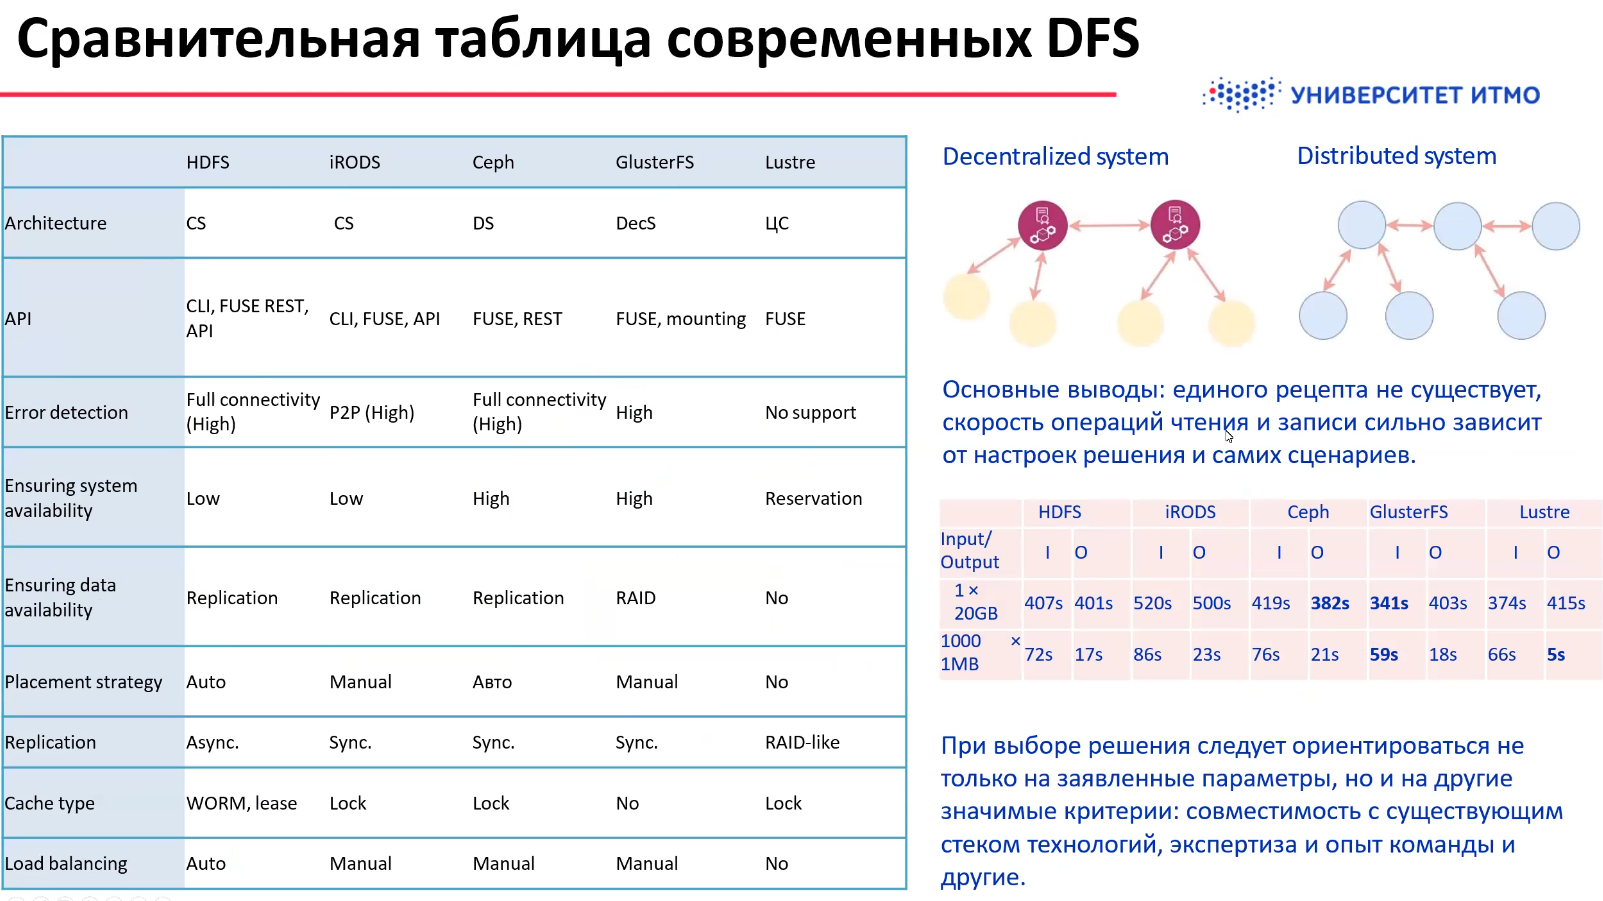
\includegraphics[width=\textwidth]{images/dfs.png}
		\caption{Сравнение DFS}
	\end{minipage}
\end{figure}

\subsection*{Облачне хранилища}

Подразумевается система с поддержкой протокола S3 (хранит объекты).

\begin{figure}[h]
	\centering
	\begin{minipage}[b]{0.8\textwidth}
		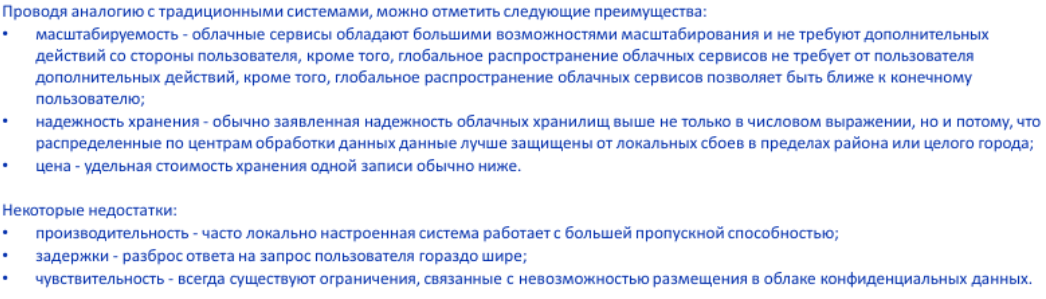
\includegraphics[width=\textwidth]{images/s3dfs.png}
		\caption{S3 vs DFS}
	\end{minipage}
\end{figure}